\chapter{Cellular Technology}
\label{chpt:celltech}
\section{Introduction}
In the current information age  almost every device has a wireless technology of sort that it uses to provide a specific service. Radios for audio entertainment; television remotes to change channels; cellular phones for communication; wireless access points to create wireless LAN's\cite{Karen2004}. Wireless technology is now part any modern human everyday life.

The popularity and rapid adoption of wireless technology has made it difficult to plan, manage and operate wireless networks\cite{Karen2004,Eisenblatter,GSMArchitectureProtocolsServices,GSM92,wirelesstelcoMullet}. Wireless technology facilitates communication between two entities by transmitting data or voice via a radio frequency\cite{Karen2004,Eisenblatter,GSMArchitectureProtocolsServices,GSM92,wirelesstelcoMullet}. 

As the popularity and use of services that use wireless technology increase, the greater the need for these services to use different radio frequencies to communicate\cite{Karen2004,Eisenblatter,GSMArchitectureProtocolsServices,GSM92,wirelesstelcoMullet}. This need arises due to an effect called \emph{interference} that occurs when two or more connections between entities use the same radio frequency to facilitate communication\cite{Karen2004,Eisenblatter,GSMArchitectureProtocolsServices,GSM92,wirelesstelcoMullet}. This effect is discussed in more detail in Chapter 3.

Therefore the use of frequencies by services must be carefully considered to avoid interference when entities communicate with each other, which is a problem since the amount of entities that communicate far out strip the amount of frequencies available for communication\cite{Karen2004,Eisenblatter,GSMArchitectureProtocolsServices,GSM92,wirelesstelcoMullet}. Thus assigning frequencies to entities for communication is a difficult problem and referred to as the frequency assignment problem (FAP)\cite{Karen2004,Eisenblatter,GSMArchitectureProtocolsServices,GSM92,wirelesstelcoMullet}.

Initially manual techniques were used to assign frequencies in an attempt to solve the FAP\cite{Karen2004,Eisenblatter,GSMArchitectureProtocolsServices,GSM92,wirelesstelcoMullet}. But as a result, the assignment of frequencies was either to complex or just too daunting because of shear amount of entities that need to be assigned frequencies\cite{Karen2004,Eisenblatter,GSMArchitectureProtocolsServices,GSM92,wirelesstelcoMullet}. Also, because of the rapid adoption of wireless technology the assignment of frequencies needed to be dynamic and hence, automated\cite{Karen2004,Eisenblatter,GSMArchitectureProtocolsServices,GSM92,wirelesstelcoMullet}.

When a task needs to be automated an algorithm needs to be developed to tell the machine how it must go about to solve the problem it is destined to work on\cite{Karen2004,Eisenblatter,GSMArchitectureProtocolsServices,GSM92,wirelesstelcoMullet}. Early algorithms developed to solve the FAP utilized brute force\footnote{Brute force refers to a method which sequentially tries every possible combination in hope of finding a solution} techniques to assign frequencies\cite{Karen2004,Eisenblatter,GSMArchitectureProtocolsServices,GSM92,wirelesstelcoMullet}.

Since the FAP is proven to be NP-Complete problem, thus using an algorithm that tries to brute force a solution is futile as no solution can be found in a reasonable time frame in chapter~\ref{chpt:fap} NP-Complete problem will defined as well as a overview of the FAP. Hence, algorithms based on heuristic techniques are utilized in an attempt to either solve the FAP or come close to a solution. Heuristic Algorithms will be discussed in Chapter 4.

In this chapter an overview of GSM networks as well as a brief history of GSM will be discussed. A discussion on the topology of GSM will then follow. This chapter will conclude with a discussion on the problems in that are present a GSM network, namely the Frequency Assignment Problem (FAP).

\section{GSM Networks}
The General System for Mobile Communications (GSM) is a system for multi-service cellular communication that is capable of providing voice as well as data services\cite{Karen2004,Eisenblatter,GSMArchitectureProtocolsServices,GSM92,wirelesstelcoMullet}. Most cellular networks in operation are GSM based\cite{Karen2004,Eisenblatter,GSMArchitectureProtocolsServices,GSM92,wirelesstelcoMullet}. The primary service that GSM caters for is voice communication, but other data services such as Short Message Service (SMS), Multimedia Message Service (MMS) and Internet connectivity services such as \emph{general packet radio system} (GPRS), \emph{enhanced data rate for global evolution} (EDGE) and \emph{high speed circuit switched data} (HSCSD) are becoming more important\cite{GSMArchitectureProtocolsServices,Eisenblatter}.

GSM is one of the most widely used radio communications technologies, which is why one needs to look at the history behind it in order to understand the domain of radio communication better \cite{GSMArchitectureProtocolsServices}. A brief history of the GSM network specification will now be presented in the next section.

\subsection{A Brief History of GSM Networks}
\label{sec:gsmhistory}
In the early 1981 a group known as the Groupe Speciale Mobile (GSM) was established to develop a Europe wide radio communication system using the reserved 900 MHz band\footnote{In 1990 the United Kingdom requested that 1800MHz band be added to the scope of the GSM standard group. This variant of the GSM specification became known as the \emph{Digital Cellular System 1800} (DCS1800) \cite{GSM92,Karen2004}.}\cite{GSM92,Karen2004}.

At the start of the GSM specification in the early 1980's it was initially thought that the system would be analogue based, but this soon changed with the \emph{integrated service digital network} (ISDN) specification nearing completion. As such the GSM specification started following much of the same design principles and access protocols that ISDN exhibited\cite{Karen2004,GSM92,GSMArchitectureProtocolsServices}.

After the completion of the ISDN specification and the advantages of switching to digital instead of analogue for communication became clear. One of the primary advantages of ISDN is that it is capable of transmitting data as higher speeds. GSM would therefore be based on digital transmission and speech would be represented by a digital stream of 16 Kbits/s \cite{Karen2004,GSM92,GSMArchitectureProtocolsServices}.

The primary benefit that one can deduce from the use of ISDN over slower analogue connections is because data can be transmitted faster, more data can be sent for the same amount of time it would've taken on an analogue connection\cite{Karen2004,GSM92,GSMArchitectureProtocolsServices}. Hence, since more data can be sent it has the net effect of increasing the quality and efficiency of the connection between two entities, the network therefore does not need to remove as much information from a packet to be sent to fit within the data transmission constraints\cite{Karen2004,GSM92,GSMArchitectureProtocolsServices}.

Before the switch to digital transmission was finalized the GSM first wanted to evaluate the spectral efficiency of analogue and digital based transmission\cite{Karen2004,GSM92,GSMArchitectureProtocolsServices}. Spectral efficiency plays an important part in wireless communication since the radio spectrum is a limited resource and whichever transmission technology is used, the utilization of the spectrum should be maximised\cite{Karen2004,GSM92,GSMArchitectureProtocolsServices}. 

Maximum utilisation is an important problem that will be discussed in detail in later sections of this chapter. After an evaluation of spectral efficiency it was finalized that the GSM system would be digitally based using \emph{time division multiple access} (TDMA) \cite{GSM92,GSMSysEngin,Eisenblatter}.

By the early 1990’s GSM became an evolving standard and the first GSM based network was demonstrated in 1991\footnote{Near the end of 1991 the GSM group was renamed to \emph{Speciale Mobile Group} (SMG) to eliminate confusion with the standard and the group}\cite{Karen2004,GSM92,GSMArchitectureProtocolsServices,Eisenblatter}. The following year a number of GSM networks were operating in Europe due to mobile terminals and equipment capable of operating on the networks becoming more widely available to the general public\cite{Karen2004,GSM92,GSMArchitectureProtocolsServices,Eisenblatter}. In the same year an operator in Australia became the first non-European operator to implement a GSM based network\cite{Eisenblatter}.

The collective subscriber base of GSM networks surpassed the million-subscriber mark in 1993. Due to this phenomenal growth in GSM network use, numerous extensions were made to the GSM specification. 
Some of the extensions that were made are the following\cite{Karen2004,GSM92,GSMArchitectureProtocolsServices,Eisenblatter}:
\begin{itemize}
\item Half rate speech telephony
\item Improved SMS
\item Line Identification
\item Call waiting
\item Call holding
\end{itemize}
The specification with these extensions defined is known as the GSM Phase 2. As the world shifted towards more digital and data intensive services it became difficult to deliver these services over GSM networks. This difficulty was due to the restriction that data could only be transmitted at 9.6 Kbps \cite{GSM92,Karen2004}.

The new specification defined new technologies such as GPRS, EDGE and HSCSD which were designed with the primary goal of making more bandwidth available for data transmission \cite{GSMArchitectureProtocolsServices,Karen2004}. Data transmission was improved by these technologies by enabling that more than one GSM slot be used for a terminal or service at a time\cite{GSMArchitectureProtocolsServices,Karen2004}.

By enabling that more than one GSM slot be used by a terminal or service, transceivers are required to have a higher signal to noise ratio \cite{GSMArchitectureProtocolsServices,GSMSysEngin}. This requirement has an impact that effects radio interfaces as there is a higher likelihood that interference might occur, hence it makes it more difficult to generate a low interference Frequency plan \cite{Eisenblatter,GSMSysEngin}. 

The actual signal to noise ratio at a receiver is dependent on a number of factors that include \cite{GSMArchitectureProtocolsServices,Karen2004}:
\begin{itemize}
\item Frequency used at the transceiver
\item Strength of the signal
\item Weather conditions
\item Shape of the surrounding environment
\item Direction of the transmission
\end{itemize}
Even taking these factors into account the calculation of the signal to noise ratio at a transceiver is not trivial. The calculation of the signal to noise ratio as well as its impact on mobile radio frequencies will be discussed in chapter~\ref{chpt:fap} section~\ref{sec:Interference}.

As the GSM standard matured as a cellular technology, industry experts already began specification of the next generation of cellular networks, which would in time, replace the GSM cellular system. 

The \emph{Universal Mobile Telecommunications System} (UMTS) can be considered the 3rd generation (3G) of cellular networks. UMTS was designed from the beginning to operate in parallel with the legacy GSM system. The first standard of the UMTS was issued in the beginning of 2000 and subsequently most modern networks are based on it or are migrating their networks to it.

UMTS is a large improvement of the GSM in two areas namely Data Transmission bandwidth and Frequency Planning due to UMTS utilising \emph{DS-CDMA} (direct sequence code division multiple access) and \emph{WCDMA} (Wide Band Code Division Multiple Access). The higher data transmission speed (2 Mb/s) can be attributed to UMTS using the DS-CDMA scheme. The scheme also allows more users to be served than previous generation of networks\cite{tabuglobalplanning3g,Eisenblatter}. 

A direct consequence of UMTS utilizing DS-CDMA and WCDMA, which sends data over a wide-band of 5 MHz, therefore no frequency planning problem comparable to GSM has to be solved\cite{tabuglobalplanning3g,Eisenblatter}. 

\emph{Code division multiple access} (CDMA) is a technology primarily used in broadband systems. Users do not gain access to only a small portion of the bandwidth, but rather use the entire band for the duration of a connection. Users also do not gain exclusive access to the whole band, but instead share the usage of the bandwidth with other users simultaneously, hence the name \emph{multiple access}. Users using a band simultaneously are separated using orthogonal codes \cite{GSMArchitectureProtocolsServices}.

With CDMA a users signal is not transmitted as its original signal. Instead the signal is spectrally spread over a multiple of its original bandwidth using a spreading factor \cite{GSMArchitectureProtocolsServices}. The spreading factor fluctuates between values of 10 and 1000 \cite{GSMArchitectureProtocolsServices}. Using these spreading factors less interference and disturbances are encountered because the broadband signal is generated from a narrowband signal \cite{GSMArchitectureProtocolsServices}.
UMTS may be a large improvement, but its adoption does not spread very far from busy city centres that contain a large concentration of clients in a small geographical area. The reason for this is that, as mentioned previously, UMTS caters for larger data usage and therefore more clients can be serviced simultaneously \cite{GSMArchitectureProtocolsServices}.

Most network operators do not implement entirely new backbone architecture for UMTS\label{UMTSGSMBackbone} to operate on but instead, utilize the same backbone used for GSM and GPRS. This not only extends the lifetime of previous infrastructure investment by the operator but also builds upon the redundancy provided by the GSM network \cite{GSMArchitectureProtocolsServices}. Thus even with new technological improvements such as UMTS, GSM as a wireless technology is still used for communication and is therefore still relevant today.

In this section a brief overview of the history of the GSM Network specification was presented. In the next section an explanation of the topology of GSM network will be given. This will broad the understanding behind GSM networks.

\begin{figure}[hptb]
	\begin{centering}
			\begin{tikzpicture}[scale=0.95]
		%\draw[step=0.25cm,thin,color=gray] (-6,-8) grid (6,8);
		%drawing of handsets
		%left handset
		\draw (-3.85,-6.20) circle (0.05cm);
		\draw (-3.85,-6.75) -- (-3.85,-6.25);
		\draw (-3.9,-8) node [below=0.15cm,right=0.005cm] {MS} rectangle (-3.15,-6.75);
		\draw (-3.8,-7.4) rectangle (-3.25,-6.8);
		\foreach \x in {0.0,0.1,0.2,0.3,0.4}
		{
			\foreach \y in {0.0,0.1,0.2,0.3}
			{
				\draw (-3.78 + \x,-7.6 - \y) rectangle (-3.68 + \x,-7.5 - \y);
			}
		}
		%right handset
		\draw (3.85,-6.20) circle (0.05cm);
		\draw (3.85,-6.75) -- (3.85,-6.25);
		\draw (3.9,-8) node [below=0.15cm,left=0.005cm] {MS} rectangle (3.15,-6.75);
		\draw (3.8,-7.4) rectangle (3.25,-6.8);
		\foreach \x in {0.0,0.1,0.2,0.3,0.4}
		{
			\foreach \y in {0.0,0.1,0.2,0.3}
			{
				\draw (3.38 + \x,-7.6 - \y) rectangle (3.28 + \x,-7.5 - \y);
			}
		}
		%Drawing of the BTS's
		\begin{scope}
			\foreach \x in {-5,-2,2,5}
			{
				\path (\x,-4.1) coordinate (TowerCirlce);
				\path (\x - 0.10,-4.215) coordinate (startLeftMast);
				\path (\x + 0.10,-4.215) coordinate (startRightMast);
				\path (\x - 0.45,-5.75) coordinate (endLeftMast);
				\path (\x + 0.45,-5.75) coordinate (endRightMast);
				\path (\x - 0.140,-4.5) coordinate (startTopHorizontalBar);
				\path (\x + 0.140,-4.5) coordinate (endTopHorizontalBar);
				\path (\x - 0.260,-5) coordinate (startMiddelHorizontalBar);
				\path (\x + 0.260,-5) coordinate (endMiddelHorizontalBar);
				\path (\x - 0.370,-5.5) coordinate (startBottomHorizontalBar);
				\path (\x + 0.370,-5.5) coordinate (endBottomHorizontalBar);
						\draw [thick,color=gray] (startLeftMast) -- (endLeftMast) (startRightMast) -- (endRightMast) (startMiddelHorizontalBar) -- (endTopHorizontalBar) -- (startTopHorizontalBar) -- (endMiddelHorizontalBar) -- (startMiddelHorizontalBar) -- (endBottomHorizontalBar) -- (startBottomHorizontalBar) -- (endMiddelHorizontalBar) -- cycle;
					\shade [ball color=gray] (TowerCirlce) circle (0.15) node [above=0.25cm] {BTS};
			}
		\end{scope}
		%Lines connecting Handsets with BTS's
		%Left
		\draw (-5,-5.75) -- (-3.9,-7.5);
		\draw (-2,-5.75) -- (-3.15,-7.5);
		%Right
		\draw (5,-5.75) -- (3.9,-7.5);
		\draw (2,-5.75) -- (3.15,-7.5);
		%Drawing of BCS's
		\begin{scope}
			\node (LeftBCS) at (-3.55,-0.75) [shape=rectangle,draw=blue!40, fill=blue!20,minimum size = 2.25cm] {BCS};
			\draw (LeftBCS.south) -- (-5,-3.35);
			\draw (LeftBCS.south) -- (-2,-3.35);
			\node (RightBCS) at (3.55,-0.75) [shape=rectangle,draw=blue!40, fill=blue!20,minimum size = 2.25cm] {BCS};
			\draw (RightBCS.south) -- (5,-3.35);
			\draw (RightBCS.south) -- (2,-3.35);
			\draw [dashed,thick,color=black] (-5.6,0.5) rectangle (5.6,-5.85) (0,0.25) node [anchor=north] {BSS System};
		\end{scope}
		%Draw MSC
		\node (MiddelMSC) at (0,2.75) [shape=rectangle,draw=black,minimum height=2.5cm, minimum width=1.5cm] {MSC};
		\draw [thick] (MiddelMSC.west) to [bend right=30] (LeftBCS.north);
		\draw [thick] (MiddelMSC.east) to [bend left=30] (RightBCS.north);
		\node (LeftMSC) at (-5,2.75) [shape=rounded rectangle,draw=black,minimum height=2.5cm, minimum width=1.5cm] {Other MSC's};
		\node (OtherNetworks) at (5,2.75) [cloud,cloud ignores aspect,cloud puffs=11,minimum height = 2.5cm,draw=black] {Other Networks};
		\draw (LeftMSC.east) to (MiddelMSC);
		\draw (MiddelMSC) to (OtherNetworks);
		%Databases
		\node (VLRDB) at (0,6.25) [cylinder,shape border rotate=90,aspect=0.45,minimum width=2cm,minimum height=1.35cm,draw] {VLR};
		\node (EIRDB) at (-4,6.25) [cylinder,shape border rotate=90,aspect=0.45,minimum width=2cm,minimum height=1.35cm,draw] {EIR};
		\node (HLRDB) at (4,6.25) [cylinder,shape border rotate=90,aspect=0.45,minimum width=2cm,minimum height=1.35cm,draw] {HLR};
		\draw[thick] (EIRDB) to [bend left=20] (MiddelMSC);
		\draw[thick] (VLRDB) to (MiddelMSC);
		\draw[thick] (HLRDB) to [bend right=20] (MiddelMSC);
		\draw[dashed,thick,color=black] (-6,8) -- (0,8) node [anchor=north] {NSS System} -- (6,8) -- (6,5) -- (2,5) -- (2,1) -- (-2,1) -- (-2,5) -- (-6,5) -- (-6,8) -- cycle;
	\end{tikzpicture}

		\caption{GSM Architecture}
		\label{fig:GSMArchitecture}
	\end{centering}
\end{figure}

\section{Topology of a GSM Network}
\label{sec:GSMArch}
A GSM networks consists of a variety of different subsystems to realise the goal of establishing a radio communication link between two parties. The hierarchy of systems and their respective connections to each other is illustrated in figure \ref{fig:GSMArchitecture}. Each subsystem will now be discussed.
\subsubsection{Mobile Station (MS)}
A Mobile station (MS) as it is defined in the GSM specification refers to any mobile device that is capable of making and receiving calls on a GSM network.  The MS is the main gateway 
for a user to gain access to the GSM network \cite{Eisenblatter,GSMArchitectureProtocolsServices}. Typical devices that fall under the category of MS are Cellular Phones, Smart Phones and Point of Sale (POS) devices. The MS has two features that play an important role throughout the GSM Network, namely:
\begin{description}
\item[Subscriber Identification Module (SIM)] --- Usually inserted into a mobile devices. The SIM contains the \emph{international mobile subscriber identity} (IMSI) and is used throughout the network for authentication as well as being a key part in providing encrypted transmissions \cite{Eisenblatter}.
\item[International Mobile Equipment Identity(IMEI)] --- Used to identify mobile station equipment. Primarily used in the denial of service to equipment that has been blacklisted\footnote{Equipment can be blacklisted for a variety of reasons e.g. theft} and tries to gain access to the network \cite{Eisenblatter}.
\end{description}
The MS has the capability to change the transmission power it uses from its base value to a maximum value of 20mW. The change in transmission power is automatically set to the lowest level by the base transceiver station (BTS) to ensure reliable communication after evaluating the signal strength as measured by the MS \cite{GSMSysEngin,GSMArchitectureProtocolsServices}. The power adjustment also minimizes cochannel interference because the transmitted signal is less powerful therefore less likely to interfere with other signals\cite{GSMSysEngin}.

\subsection{Base Station Subsystem (BSS)}

According to the GSM Phase 2+ specification this system is viewed by the \emph{mobile switching centre} (MSC) through an Abis radio interface as the system responsible for communicating with mobile stations in a particular location area \cite{Eisenblatter}. The BSS usually consists of one \emph{base station controller} (BSC) with one or more \emph{base transceiver stations} (BTS) that it controls \cite{Eisenblatter}. The communication link between the MSC and BSC is the called the A-interface and the communication link between the BSC and BTS is called the Abis interface \cite{Eisenblatter}. A BTS has similar equipment to that of a Mobile Station \cite{GSMSysEngin}. Both have transceivers, antennas and the necessary functions to perform radio communication. 

Communication between the various GSM entities occurs over these interfaces via radio channels, which are in fact, certain frequencies that are used to transmit information wirelessly. A more in depth discussion on the type of channels that are in defined and used in a GSM network as well as their purpose will be presented in section \ref{sec:interfacech}.

In a GSM network the Service Area (SA) is subdivided into Location Areas (LAs) which are then further divided into smaller radio zones called cells \cite{GSMSecurInTeleNetwork}. When a cellular network is modelled, cells are modelled as hexagonal shapes. Each cell in the modelled network is served by only one BTS\footnote{Also referred to as a Site} and is usually regarded to be in the centre of a cell as can be seen in figure \ref{fig:GSMCell}\cite{GSMArchitectureProtocolsServices}. Even though cells are modelled as being hexagons (see figure \ref{fig:GSMCell}) the actual coverage area of a cell has no predefined regular shape \cite{GSMArchitectureProtocolsServices}.

With the network modelled as a series of interconnecting hexagons it allows one to more easily take constraints into account. For a cell to serve its geographical area, it needs to be allocated frequencies to operate on. Therefore, for each cell $i$ in the modelled network a subset $S_i$ of frequencies from the total frequencies $F$ allocated to the GSM network is assigned\cite{GSMArchitectureProtocolsServices}. Neighbouring cells must at all cost avoid having the same subset of frequencies allocated to them, since such a scenario would lead to severe interference on any communication and thus degrade quality \cite{GSMArchitectureProtocolsServices}.
Since the amount of cells in a network greatly outnumber the available of subset frequencies available one is forced to start reusing frequency subsets in cells. To ensure the reused frequency subsets do not interfere with their neighbouring cells a reuse distance $D$ is defined \cite{GSMArchitectureProtocolsServices}. Which basically means that a certain amount of cells must be between the cell already assigned the frequency subset $S_i$ and the cell to be assigned a frequency subset \cite{GSMArchitectureProtocolsServices}. The amount of cells is the distance value $D$.

The size of a cell determines the amount of potential traffic that cell will be required to handle \cite{GSM92,Eisenblatter,GSMArchitectureProtocolsServices}. Therefore, if the size of a cell is chosen to be small, less channels will be required to be allocated to that cell as it would not be required to handle that much traffic as a larger cell. 

By making the size of cells smaller, the network operator is required to invest more into its network infrastructure. Smaller cells has a direct consequence that more cells would be required to serve the same geographical area and more cells means more BTS's etc. need to be built and maintained, not to mention that more BTSs also means more locations need to be rented \cite{GSMArchitectureProtocolsServices}. Hence, making a cell smaller has a compounding effect on the amount of infrastructure needed to support it.

Fortunately all the extra infrastructure investment by the operator can be greatly scaled down if cells are divided into sectors\label{def:cellsector}. Each sector performs the exact same function as a traditional cell and is therefore regard to also be a cell just smaller in size and not omni-directional \cite{GSMArchitectureProtocolsServices,GSM92,GSMSysEngin}. 

A cell is divided into 3 to 6 service sectors and each sector is allocated an antenna/transceiver \cite{GSMSysEngin}. Depending on how many sectors are at a cell, the operating angle of the antennae needs to be adjusted accordingly to ensure 360 degree service. If there is only one sector an omni-directional antenna is used, otherwise the antennae operating angle are adjusted to $\frac{360\,^{\circ}}{n}$ where ${n}$ is the amount of antennae \cite{Eisenblatter}.
\begin{figure}[t!]
	\begin{centering}
		\begin{tikzpicture}
	%===============================Top======================================
	\node [regular polygon, regular polygon sides=6, minimum size=3cm,draw] at (0,1) {};
	\path (0,1.75) coordinate (TowerCirlce);
	\path (0 - 0.10,1.635) coordinate (startLeftMast);
	\path (0 + 0.10,1.635) coordinate (startRightMast);
	\path (0 - 0.45,0.01) coordinate (endLeftMast);
	\path (0 + 0.45,0.01) coordinate (endRightMast);
	\path (0 - 0.140,1.345) coordinate (startTopHorizontalBar);
	\path (0 + 0.140,1.345) coordinate (endTopHorizontalBar);
	\path (0 - 0.260,0.85) coordinate (startMiddelHorizontalBar);
	\path (0 + 0.260,0.85) coordinate (endMiddelHorizontalBar);
	\path (0 - 0.370,0.35) coordinate (startBottomHorizontalBar);
	\path (0 + 0.370,0.35) coordinate (endBottomHorizontalBar);
	\draw [thick,color=gray] (startLeftMast) -- (endLeftMast) (startRightMast) -- (endRightMast) (startMiddelHorizontalBar) -- (endTopHorizontalBar) -- (startTopHorizontalBar) -- (endMiddelHorizontalBar) -- (startMiddelHorizontalBar) -- (endBottomHorizontalBar) -- (startBottomHorizontalBar) -- (endMiddelHorizontalBar) -- cycle;
	\shade [ball color=gray] (TowerCirlce) circle (0.15) node [above=0.10cm] {\tiny{BTS}};
	%%========================================================================
	%%================================Second Line======================================
	\foreach \x in {-2.25,2.25}
	{
		\node [regular polygon, regular polygon sides=6, minimum size=3cm,draw] at (\x,-0.3) {};
		\path (\x,-0.3 + 0.75) coordinate (TowerCirlce);
		\path (\x - 0.10,-0.3 + 0.635) coordinate (startLeftMast);
		\path (\x + 0.10,-0.3 + 0.635) coordinate (startRightMast);
		\path (\x - 0.45,-0.3 - 0.99) coordinate (endLeftMast);
		\path (\x + 0.45,-0.3 - 0.99) coordinate (endRightMast);
		\path (\x - 0.140,-0.3 + 0.345) coordinate (startTopHorizontalBar);
		\path (\x + 0.140,-0.3 + 0.345) coordinate (endTopHorizontalBar);
		\path (\x - 0.260,-0.3 - 0.15) coordinate (startMiddelHorizontalBar);
		\path (\x + 0.260,-0.3 - 0.15) coordinate (endMiddelHorizontalBar);
		\path (\x - 0.370,-0.3 - 0.65) coordinate (startBottomHorizontalBar);
		\path (\x + 0.370,-0.3 - 0.65) coordinate (endBottomHorizontalBar);
		\draw [thick,color=gray] (startLeftMast) -- (endLeftMast) (startRightMast) -- (endRightMast) (startMiddelHorizontalBar) -- (endTopHorizontalBar) -- (startTopHorizontalBar) -- (endMiddelHorizontalBar) -- (startMiddelHorizontalBar) -- (endBottomHorizontalBar) -- (startBottomHorizontalBar) -- (endMiddelHorizontalBar) -- cycle;
		\shade [ball color=gray] (TowerCirlce) circle (0.15) node [above=0.10cm] {\tiny{BTS}};
	}
	%%========================================================================
	%%================================Third Line======================================
	\node [regular polygon, regular polygon sides=6, minimum size=3cm,draw] at (0,-1.6) {};
	\path (0,-1.6 + 0.75) coordinate (TowerCirlce);
	\path (0 - 0.10,-1.6 + 0.635) coordinate (startLeftMast);
	\path (0 + 0.10,-1.6 + 0.635) coordinate (startRightMast);
	\path (0 - 0.45,-1.6 - 0.99) coordinate (endLeftMast);
	\path (0 + 0.45,-1.6 - 0.99) coordinate (endRightMast);
	\path (0 - 0.140,-1.6 + 0.345) coordinate (startTopHorizontalBar);
	\path (0 + 0.140,-1.6 + 0.345) coordinate (endTopHorizontalBar);
	\path (0 - 0.260,-1.6 - 0.15) coordinate (startMiddelHorizontalBar);
	\path (0 + 0.260,-1.6 - 0.15) coordinate (endMiddelHorizontalBar);
	\path (0 - 0.370,-1.6 - 0.65) coordinate (startBottomHorizontalBar);
	\path (0 + 0.370,-1.6 - 0.65) coordinate (endBottomHorizontalBar);
	\draw [thick,color=gray] (startLeftMast) -- (endLeftMast) (startRightMast) -- (endRightMast) (startMiddelHorizontalBar) -- (endTopHorizontalBar) -- (startTopHorizontalBar) -- (endMiddelHorizontalBar) -- (startMiddelHorizontalBar) -- (endBottomHorizontalBar) -- (startBottomHorizontalBar) -- (endMiddelHorizontalBar) -- cycle;
	\shade [ball color=gray] (TowerCirlce) circle (0.15) node [above=0.10cm] {\tiny{BTS}};
	%%========================================================================
	%%================================Fourth Line======================================
	\foreach \x in {-2.25,2.25}
	{
		\node [regular polygon, regular polygon sides=6, minimum size=3cm,draw] at (\x,-2.9) {};
		\path (\x,-2.9 + 0.75) coordinate (TowerCirlce);
		\path (\x - 0.10,-2.9 + 0.635) coordinate (startLeftMast);
		\path (\x + 0.10,-2.9 + 0.635) coordinate (startRightMast);
		\path (\x - 0.45,-2.9 - 0.99) coordinate (endLeftMast);
		\path (\x + 0.45,-2.9 - 0.99) coordinate (endRightMast);
		\path (\x - 0.140,-2.9 + 0.345) coordinate (startTopHorizontalBar);
		\path (\x + 0.140,-2.9 + 0.345) coordinate (endTopHorizontalBar);
		\path (\x - 0.260,-2.9 - 0.15) coordinate (startMiddelHorizontalBar);
		\path (\x + 0.260,-2.9 - 0.15) coordinate (endMiddelHorizontalBar);
		\path (\x - 0.370,-2.9 - 0.65) coordinate (startBottomHorizontalBar);
		\path (\x + 0.370,-2.9 - 0.65) coordinate (endBottomHorizontalBar);
		\draw [thick,color=gray] (startLeftMast) -- (endLeftMast) (startRightMast) -- (endRightMast) (startMiddelHorizontalBar) -- (endTopHorizontalBar) -- (startTopHorizontalBar) -- (endMiddelHorizontalBar) -- (startMiddelHorizontalBar) -- (endBottomHorizontalBar) -- (startBottomHorizontalBar) -- (endMiddelHorizontalBar) -- cycle;
		\shade [ball color=gray] (TowerCirlce) circle (0.15) node [above=0.10cm] {\tiny{BTS}};
	}
	%%========================================================================
	%%================================Fifth Line======================================
	\node [regular polygon, regular polygon sides=6, minimum size=3cm,draw] at (0,-4.2) {};
	\path (0,-4.2 + 0.75) coordinate (TowerCirlce);
	\path (0 - 0.10,-4.2 + 0.635) coordinate (startLeftMast);
	\path (0 + 0.10,-4.2 + 0.635) coordinate (startRightMast);
	\path (0 - 0.45,-4.2 - 0.99) coordinate (endLeftMast);
	\path (0 + 0.45,-4.2 - 0.99) coordinate (endRightMast);
	\path (0 - 0.140,-4.2 + 0.345) coordinate (startTopHorizontalBar);
	\path (0 + 0.140,-4.2 + 0.345) coordinate (endTopHorizontalBar);
	\path (0 - 0.260,-4.2 - 0.15) coordinate (startMiddelHorizontalBar);
	\path (0 + 0.260,-4.2 - 0.15) coordinate (endMiddelHorizontalBar);
	\path (0 - 0.370,-4.2 - 0.65) coordinate (startBottomHorizontalBar);
	\path (0 + 0.370,-4.2 - 0.65) coordinate (endBottomHorizontalBar);
	\draw [thick,color=gray] (startLeftMast) -- (endLeftMast) (startRightMast) -- (endRightMast) (startMiddelHorizontalBar) -- (endTopHorizontalBar) -- (startTopHorizontalBar) -- (endMiddelHorizontalBar) -- (startMiddelHorizontalBar) -- (endBottomHorizontalBar) -- (startBottomHorizontalBar) -- (endMiddelHorizontalBar) -- cycle;
\shade [ball color=gray] (TowerCirlce) circle (0.15) node [above=0.10cm] {\tiny{BTS}};
\end{tikzpicture}

		\caption{Cells with BTS's}
		\label{fig:GSMCell}
	\end{centering}
\end{figure}

By dividing the cell into sectors the amount of co-channel interference that would occur in a cell is greatly reduced \cite{GSMArchitectureProtocolsServices}. It is important to note that the reduction of co-channel interference is only applicable when the angle of the anttenaue by which transmission occurs is restricted\cite{GSMArchitectureProtocolsServices}.

For instance, if a cell using an omni-directional transceiver is assigned 6 channels. If the cell were to be divided into 3 sectors, where the sectors antennae are $120^\circ$ apart, the amount of interfering co-channels shrink from 6 to 2 and from 6 to 1 in the case that the cell is divided into 6 sectors \cite{GSMSysEngin,GSM92,GSMArchitectureProtocolsServices}.

\begin{figure}[t!]
	\begin{centering}
	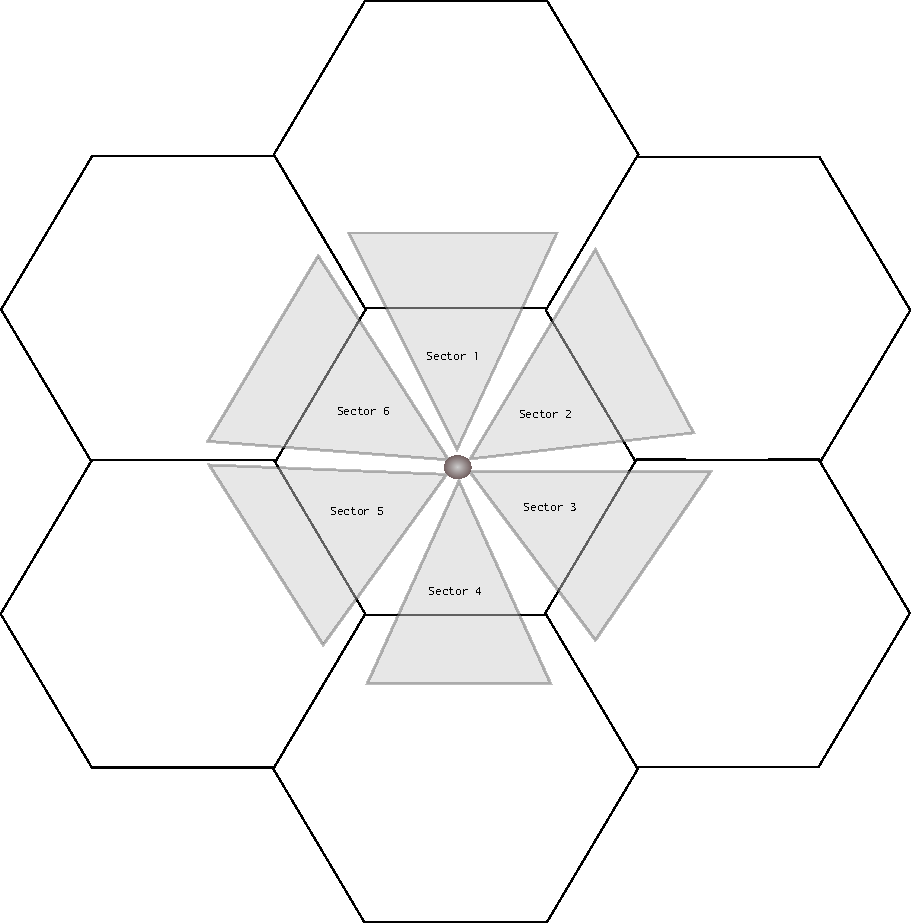
\includegraphics[scale=0.75]{tikz-pics/cellsector.pdf}
	\label{fig:cellsector}
	\caption[Cell Sectorization]{A cell that has been divided into sectors is illustrated. It can be observed that the center cell has been sectorized into 6 distinct sectors using directional tranceivers. With the a traceiver servicing each sector it can be seen in the figure that the tranceiver will interfere only one cell.}
	\end{centering}
\end{figure}

Each sector operates one or more elementary transceivers called TRX’s. The amount of TRX’s per sector is determined by the expected peak traffic demand that the cell must be able to handle. Each TRX can handle 7 to 8 communication links or calls in parallel except the first TRX, which handles fewer calls than normal due to it being responsible for transmitting cell organisation and protocol information \cite{Eisenblatter}. TRX’s are able to handle 7-8 calls in parallel due to the use of \emph{frequency division multiplexing} (FDM) and \emph{time division multiplexing} (TDM) schemes. 

TRX’s are assigned channels, which enable them to provide conversion between digital traffic data on the network side and the radio communication between Mobile Stations and the GSM network\cite{ACOvsEA,FAPOrientationModel}. The various channels that are used by a cell for communication are discussed in section \ref{sec:interfacech}.

\subsection{Mobile Switching Centre (MSC)}

The MSC is at the heart of cellular switching system and forms part of the \emph{Network Switching Subsystem} (NSS). The MSC is responsible for the setting up, routing and supervision of calls between GSM subscribers\cite{GSM92,GSMSysEngin}. The MSC has interfaces on the one side to communicate with GSM subscribers (through the BSS) and on the other it has interfaces to communicate with external networks\cite{GSM92}. The MSC interfaces with external networks to utilise their superior capability in data transmission as well as for the signalling and communication with other GSM entities \cite{GSM92}. 

The most basic functions that an MSC is responsible for in a network are the following \cite{wirelesstelcoMullet}:
\begin{itemize}
\item Voice call initialization, routing, control and supervision between subscribers.
\item Handover process between two cells.
\item Location updating.
\item MS authentication.
\item SMS delivery.
\item Charging and Accounting of services used by subscriber.
\item Notification of other network elements.
\item Administration input or output processing functions.
\end{itemize}

To achieve most of these functions the MSC has an integrated \emph{Visitor Location Register (VLR)} database that stores call setup information for any MS that is currently registered for service with the MSC \cite{GSM92,wirelesstelcoMullet}. 

The VLR retrieves this information from the \emph{Home Location Register (HLR)} that contains all the registered GSM subscriber information for the network. This information enables the MSC to quickly retrieve the necessary information to setup a call between two entities \cite{GSMSysEngin,GSMSecurInTeleNetwork}.

A requirement for being able to communicate with other network elements such as \emph{Public Switching Telephone Networks} (PSTN) is the ability to multiplex and demultiplex signals to and from such network elements. This operation is a necessity, since the incoming or outgoing connection bitrate from the source entity might either be to low or to high for the receiving entity.

A typical scenario where this operation proves vital is when a mobile subscriber makes a call to a subscriber on a PSTN. The connection bit rate needs to be changed at the MSC from a wireless connection bitrate to a bitrate suitable for transmission over a PSTN.

\subsection{Network Databases}
The HLR, AUC (Authentication Centre) and EIR (Equipment Identity Register) are the three 'back-end' databases, which stores and provides information for the rest of the GSM Network. In this subsection each one of the databases that form part of the 'back-end' will be briefly discussed as well as a description will be given of the core functions that each database performs in the network.

\paragraph{Home Location Register (HLR)}
The HLR is a database that permanently stores information pertaining to a given set of subscribers. The HLR needs to store a wide range of subscriber parameters because it is the reference source for anything GSM subscriber related in the network. 

Subscriber parameters that are stored in the database include: Billing information, routing information, identification numbers, authentication parameters, subscribed services. The following information is also stored but the information is of a temporary nature and can change at any time: Current VLR and MSC the subscriber is registered with; whether the subscriber is roaming \cite{GSMSysEngin}.

\paragraph{Authentication Centre (AUC)}
The Authentication center is the entity in the GSM network that performs security functions and thus stores information that enables it to provide secure over the air communication\cite{GSM92,GSMSysEngin}. The information that is stored contains authentication information as well as keys that are used in ciphering of information\cite{GSM92,GSMSysEngin}.

During an authentication procedure no ciphering key is ever transmitted over the air, instead a challenge is issued to the mobile that needs to be authenticated. This challenge requires the mobile station to provide the correct \emph{Signed Response} (SRES) with regard to the random number generated by the AUC\cite{GSM92,GSMSysEngin}. The random number and ciphering keys that are used change with each call that is made, thus an attacker would gain nothing by intercepting a key, since it will change with the next call \cite{GSMSysEngin}.

Each mobile that is registered in the HLR database needs to be authenticated and each call that is instantiated needs to retrieve keys from the AUC to establish a secure communication link\cite{GSM92,GSMSysEngin}. The AUC is sometimes included with HLR to allow for fast communication between the two entities \cite{GSMSysEngin}.

\paragraph{Equipment Identity Register (EIR)}
The EIR is a database that stores the IMEI numbers of all registered mobile equipment that has accessed the network. Only information about the mobile equipment is stored, nothing about the subscriber or call is stored in the database.

Typically there is only one EIR database per network and interfaces to the various HLR database contained in the network. The IMEI's are grouped into three categories: \emph{White List}, \emph{Black List} and the \emph{Gray List}. The White list contains only the IMEI numbers of valid MS's; the Black List stores the IMEI numbers of equipment that has been reported stolen and the Gray List stores the IMEI numbers of equipment that has some fault (faulty software, wrong make of equipment).

\subsection{GSM Network Management entities}
In a GSM network most of the elements that form part of and make the network function are often distributed in a wide geographical area to provide the best network coverage for the customer. 

For a network to function properly and efficiently network engineers need to be kept up to date on the state of the network and be alerted if \emph{any} problems occur. For this purpose there exist two systems in the GSM network architecture that allows for this functionality required by network engineers. 

The one system is called the Operations and Management centre which is responsible for centralized regional and local operational and maintenance activities. The other system called the Network Management System unlike the OMC provides global and centralized management for operations and maintenance of the network supposed by the OMCs \cite{GSMSysEngin}.

In the following sections a more indepth discussion on the critical functions the OMC and NMC perform will be presented.

\paragraph{Operational and Management Centre}
The OMC is capable of communicating with GSM entities using two protocols namely SS7 and X.25. The SS7 protocol is usually used when the OMC is communicating within the GSM network over short and medium distances. The X.25 protocol is used for large external data transfers. All communication where the OMC is involved typically occurs over fixed line networks and/or leased lines. The OMC is usually used for day to day operation of a network \cite{GSMSysEngin}.

The OMC has support for alarm handling. An alarm in a GSM network goes of whenever a predefined expected condition does occurs. Engineers are able to define the severity of an alarm, which defines who and what is further, alerted when and if the alarm is escalated to a higher level \cite{GSMSysEngin}.

The OMC is also capable of fault management in the GSM network. The OMC is able to activate, deactivate, remove and restore a service manually or automatically of network devices\cite{GSM92}. Various tests can be run as well as diagnostic information can be retrieved on the network devices to detect any current or future defects \cite{GSMSysEngin}.

\paragraph{Network Management Centre}
The NMC is similar to the OMC but it is not restricted to only regional GSM entities as it is in charge of the all GSM entities in the network. The NMC provides traffic management for the global network and also monitors high priority alarms such as overloaded or failed network nodes. It is usually used in long term planning of a network, but it has the capability to perform certain OMC functions when an OMC is not staffed. 

\section{GSM Interfaces}
\label{sec:gsminterfaces}
In the GSM network all the various entities communicate with each other through various pre-defined interfaces. In this section an overview will be presented on these various interfaces that exist between the entities.
\begin{description}
\item{\textbf{Um Interface}} --- This interface is the link between a MS entity and a BTS and is also referred to as the \emph{Air} interface since communication occurs wirelessly. The primary protocol used on this interface is the LAPDm, which is an extension to the ISDN LAPD protocol to accommodate the mobile nature of MS devices as well as for the shorter TDMA frames which are used in GSM networks\cite{wirelesstelcoMullet,GSMSecurInTeleNetwork}.
\item{\textbf{Abis Interface}} --- Between the BTS and BSC the interface used for communication is known as the Abis interface. The only messages that the BTS are interested in are those that have to do with management of radio resources\cite{wirelesstelcoMullet,GSMSecurInTeleNetwork}. All other messages are left alone and merely pass through the BTS to the BSC transparently.
\item{\textbf{A Interface}} --- The interface between the BSC and MSC is known as the A interface. This interface is used for the transfer of information, which is used by the MSC to manage BSSs, control connections and to manage the mobility of MS in its administrative area \cite{wirelesstelcoMullet,GSMArchitectureProtocolsServices}.
\item{\textbf{Other Interfaces}} --- The MSC has various interfaces going from itself to the various databases and other external network. Each interface connects to a specific database,MSC or network and is therefore very specific as to what function it performs\cite{wirelesstelcoMullet,GSMArchitectureProtocolsServices}. An interface going from one MSC to another MSC will typically convey information regarding handling the administration of handover a MS device leaving the one administrative area to another MSC's administrative area. The handover procedure is a very delicate process which will be described in section \ref{sec:handover}.
\end{description}

In this section a brief overview of the most critical interfaces used by all the involved entities of the GSM network was presented. In the next section a discussion will be given describing the difference between a logical channel and a frequency. Additionally an outline and overview of all the logical channels defined in the GSM will be presented. 
\section{GSM Channels}
\label{sec:interfacech}
GSM defines a series of logical channels, which are used for communication over these interfaces. A distinction needs to be made between channels and frequencies. As discussed earlier, a network is licensed a certain section of the wireless spectrum for use for commercial communication. This piece of spectrum is referred to as bandwidth and is measured in Hz, therefore $W$ Hz, where $W$ denotes the allocated bandwidth\cite{FundamentalsWirelessCommunication}.

This bandwidth W is then divided into N smaller chunks of bandwidth called narrowband chunks. Each N narrowband chunk is a channel and has a width of $W/N$ Hz\cite{FundamentalsWirelessCommunication}. This channel of $W/N$ Hz width is also referred to as a frequency.\label{def:channel}

The terms channel and frequency can therefore be used interchangeably. In this dissertation the term channel will be used.

Using TDMA the GSM system is able to provide additional transmission capacity by dividing the channel into eight equal time slots \cite{wirelesstelcoMullet}. 
\begin{figure}[h]
	\begin{centering}
		\begin{tikzpicture}[]
	\begin{scope}[node distance=0cm]
		\node (startSquare) at (-6.0,0.5) [shape=rectangle,draw=black,minimum height = 0.75cm,minimum width = 0.8cm]{   };
		\node (secondSquare) [right = of startSquare,shape=rectangle,draw=black,minimum height = 0.75cm,minimum width = 0.8cm]{   };
		\node (TS0) [right = of secondSquare, shape=rectangle,draw=black,fill=gray!40,minimum height = 0.75cm,minimum width = 0.8cm]{TS1};
		\node (TS1) [right = of TS0, shape=rectangle,draw=black,fill=gray!40,minimum height = 0.75cm,minimum width = 0.8cm]{TS2};
		\node (TS2) [right = of TS1, shape=rectangle,draw=black,fill=gray!40,minimum height = 0.75cm,minimum width = 0.8cm]{TS3};
		\node (TS3) [right = of TS2, shape=rectangle,draw=black,fill=gray!40,minimum height = 0.75cm,minimum width = 0.8cm]{TS4};
		\node (TS4) [right = of TS3, shape=rectangle,draw=black,fill=gray!40,minimum height = 0.75cm,minimum width = 0.8cm]{TS5};
		\node (TS5) [right = of TS4, shape=rectangle,draw=black,fill=gray!40,minimum height = 0.75cm,minimum width = 0.8cm]{TS6};
		\node (TS6) [right = of TS5, shape=rectangle,draw=black,fill=gray!40,minimum height = 0.75cm,minimum width = 0.8cm]{TS7};
		\node (TS7) [right = of TS6, shape=rectangle,draw=black,fill=gray!40,minimum height = 0.75cm,minimum width = 0.8cm]{TS8};
		\node (secondLastSquare) [right = of TS7, shape=rectangle,draw=black,minimum height = 0.75cm,minimum width = 0.8cm]{   };
		\node (lastSquare) [right = of secondLastSquare, shape=rectangle,draw=black,minimum height = 0.75cm,minimum width = 0.8cm]{   };
	\end{scope}
	\node (startF) at (startSquare.west) [above=1.5cm]{};
	\node (endF) at (lastSquare.east) [above=1.5cm]{};
	\draw [|<->|,thick] (startF) to node [above=0.05cm] {Frequency} (endF);
	\draw[decorate,decoration={brace,amplitude = 0.5cm,raise=0.5cm}] (TS0.west) to node [above=1cm] {TDMA Frame} (TS7.east);
	\node (logicalChannel) [shape=rectangle,draw=black,below = 1.5cm of TS4] {Logical Channel};
	\draw (logicalChannel.north east) to (TS1.south east);
	\draw (logicalChannel.north west) to (TS1.south west);
\end{tikzpicture}

		\caption{TDMA Frame and Logical channels \cite{wirelesstelcoMullet}}
		\label{fig:GSMChannels}
	\end{centering}
\end{figure}
As can be observed from figure \ref{fig:GSMChannels} each TDMA frame has a series of consecutive timeslots. Each timeslot can be used for both uplink and downlink transmission. A GSM \emph{channel} is a logical channel and refers to a single timeslot within a TDMA frame \cite{wirelesstelcoMullet,GSMArchitectureProtocolsServices}.

The GSM system is hence able to use the same physical frequency in eight different timeslots without interference as these \emph{logical} channels are used at different times. Therefore using TDMA the available channels that can be used for communication in GSM is increased eight fold \cite{wirelesstelcoMullet}.

Frequencies are assigned to the uplink and downlink portion of the connection with a certain duplex separation in the frequency band \footnote{Separation is usually 45 MHz} to avoid interference between uplink and downlink. There are two types of channels, traffic channels and control channels. Traffic channels (TCHs) primary purpose is to enable communication of user speech and data and therefore carry no control information \cite{GSMArchitectureProtocolsServices}.

A TCH is assigned to a MS device when the device requests that it needs to communicate with another device either with speech or data. When a MS is done with the TCH the allocated TCH is reclaimed for use by other MS devices on the network. This request by the MS device occurs using over the control channels \cite{GSMArchitectureProtocolsServices}.

Control channels are much more actively used in a GSM network since it is the primary means by which control and management of the network occurs \cite{GSMArchitectureProtocolsServices}. These channels are used even when the MS has no active connection and is hence in idle mode. This constant activity on the control channels is to keep the network update with information such as the position of the MS (location updating) and signal strength \cite{GSMArchitectureProtocolsServices,GSMSysEngin,Eisenblatter}. 

The control channels are divided into three main channel groups namely Broadcast Channel (BCH), Common Control Channel (CCCH) and Dedicated Control Channel (DCCH) \cite{GSMArchitectureProtocolsServices}. Each of these channel groups contains furthermore channels that aid in the control and management of the network. Each group along with the associated channels shall now be briefly discussed.

The first group, BCH consists of three channels:
\begin{description}
\item{\textbf{Broadcast Control Channel (BCH)}} --- This channel is broadcasted using the very first frequency assigned to a cell. Using this frequency, the channel broadcasts information regarding the network. This information includes radio channel configuration of the current and neighbouring cells; synchronization information, registration identifiers and most importantly the format of the CCH used by the local BTS \cite{GSMArchitectureProtocolsServices}.
\item{\textbf{Frequency Correction Channel (FCCH)}} --- Synchronization information is broadcasted to the MSs to enable them to perform frequency correction on the transmission. Typical synchronization information on this channel for instance, is the exact frequency the local BTS is using for transmission to enable the MSs attune itself to the same frequency \cite{GSMArchitectureProtocolsServices}.
\item{\textbf{Synchronization Channel (SCH)}} --- On this channel, identifying information regarding the BTS is transmitted. Also, also on this channel information regarding synchronization of frames is sent which aids a MS to for example to structure the time frames of TDMA frames.
\end{description}

The FCCH and SCH are always broadcasted with the BCH since these channels are needed for operation of the radio subsystem \cite{GSMArchitectureProtocolsServices}. The CCCH is a point-to-point signalling channel that is used to localize a MS with the use of paging. The channel is also used to assign dedicated channels \cite{GSMArchitectureProtocolsServices}. The CCCH is made up of the following channels:
\begin{description}
\item{\textbf{Random Access Channel (RACH)}} --- RACH forms the uplink portion of the CCH channel and is randomly accessed by the MSs to request a dedicated channel for a single signalling transaction \cite{GSMArchitectureProtocolsServices}.
\item{\textbf{Access Grant Channel (AGCH)}} --- AGCH from the downlink part of the CCH channel. It is used by the radio subsystem to assign a SDCCH or TCH to a MS \cite{GSMArchitectureProtocolsServices}.
\item{\textbf{Paging Channel (PCH)}} --- PCH also forms part of the downlink portion of the CCH channel. This channel is used by the radio subsystem to page specific MSs, which aids in the process of locating a MS \cite{GSMArchitectureProtocolsServices}.
\item{\textbf{Notification Channel (NCH)}} --- This channel is used to inform an MS of any incoming group calls or calls that is being broadcasted \cite{GSMArchitectureProtocolsServices}.
\end{description}

The last group of signalling channels are referred to as Dedicated/Associated Control Channels (D/ACCH). These groups of channels have the characteristic that they are bidirectional point to point channels \cite{GSMArchitectureProtocolsServices}.
\begin{description}
\item{\textbf{Stand-alone Dedicated Control Channel}} --- This channel is used for communication between the BSS and MS even when there is no active connection. Hence the 'stand-alone' since it means that there need not be a TCH assigned for communication to occur between the BSS and MS \cite{GSMArchitectureProtocolsServices}.
\item{\textbf{Slow Associated Control Channel (SACCH)}} --- When a TCH or SDCCH is assigned, there must be accompanied SACCH also assigned. The SACCH is used to transmit information for optimal radio operation, which can include information on power control of the radio transmitter and synchronization information. Packets must be continuously sent over the SACCH as it is used as proof that there is still a physical radio connection \cite{GSMArchitectureProtocolsServices}. When the MS is done using the SACCH channel, it transmits a report regard the current results of the radio signal level, which is continuously measured \cite{GSMArchitectureProtocolsServices}.
\item{\textbf{Fast Associated Control Channel (FACCH)}} --- When more bandwidth is required for signalling purposed, the signal of the TCH is modified using dynamic pre-emptive multiplexing. The additional bandwidth comes at the expense of the user date transport. When a channel is created in this manner it is called a FACCH \cite{GSMArchitectureProtocolsServices}.
\end{description}

Finally, one last channel is defined named the Cell Broadcast Channel (CBCH), which shares the same physical channel that the SDCCH uses. On this channel messages of the Short Message Service Cell Broadcast are broadcasted \cite{GSMArchitectureProtocolsServices}.

In this section a section an overview was given on how \emph{logical} channels used for communication between a MS and BSS/MSC. These three groups of channels collectively enable the GSM network to facilitate wireless communication, a very important function for a telecommunication network. In the following section a discussion will be presented on how the network is able to keep a connection to a MS alive and allow the MS to make calls while the device is moving around geographically within the network.
\section{Handover}
\label{sec:handover}
In this section a discussion will be given describing the process GSM network entities go through when a handover needs to occur. The Handover process in a GSM network is initiated when a MS with an active call moves outside the coverage area of a cell, BSS or MSC \cite{GSMArchitectureProtocolsServices,wirelesstelcoMullet,Eisenblatter}. Besides the MS moving outside the coverage area, a handover might also be initiated because of measurements indicating bad channel quality\cite{GSMArchitectureProtocolsServices}. 

Various information needs to be migrated across and shared between the entities to ensure a smooth handover, which results in the MS active call not suddenly ending. It is just not the GSM architecture entities that need to continuously share information but also the MS. The MS is required to continuously observe and measure signal strength of up to 6 neighbouring cells. The MS does this by monitoring the BCCH\cite{GSMArchitectureProtocolsServices,wirelesstelcoMullet}. This information is of course relayed to the MSC and BTS as it plays a critical role in the decision process as to which entity will be the best in taking over the administration of the active call\cite{GSMArchitectureProtocolsServices,wirelesstelcoMullet}.

A MS can in some cases receive the same BCCH from different cells, which are most likely neighbours \cite{GSMArchitectureProtocolsServices}. This problem of duplicate BCCH from different cells can be attributed to the frequency reuse in the cellular network as well as due to the smaller sector cells forming clusters and therefore overlapping coverage area \cite{GSMArchitectureProtocolsServices}. As discussed in section \ref{def:cellsector} page \pageref{def:cellsector}, cells are typically divided into sectors, which lessen the problem of co-channel interference. This division into sectors can cause clustering of cells and overlapping of coverage area.

This forms a problem for the MS since the it needs to distinguish between the two cells measurements as it does not know which measurement belongs to what cell \cite{GSMArchitectureProtocolsServices}. To distinguish between different cells, the MS also tries to determine the identity of each cell it is monitoring. Only cells whose identity can be reliably determined are included in the report sent to the BTS\cite{Eisenblatter,GSMArchitectureProtocolsServices,wirelesstelcoMullet}\footnote{Cells whose identity can't be determined can be due to environmental factors like signal strength or to packets getting lost/dropped}. Using this report the handover algorithm is able to decide how to handle the handover, which cell needs to take over the call\cite{Eisenblatter,GSMArchitectureProtocolsServices,wirelesstelcoMullet}.

Once the cell has been selected, the actual handover process starts. Which has to take into account that the frequency allocated to the incoming call from the other cell does not interfere with other present active calls in the cell receiving the handover\cite{Eisenblatter,GSMArchitectureProtocolsServices,wirelesstelcoMullet}. A frequency interfering with calls currently active in the cell can cause users to hear other conversations from the interfering call, or experience their call being ``dropped'' i.e. disconnected\cite{Eisenblatter}. 

There are three core handover procedures when a handover needs to occur in a GSM network. \emph{Intra-BSC}, \emph{Inter-BSC} and \emph{Inter-MSC} each of which involves different GSM entities \cite{wirelesstelcoMullet}. A brief discussion on each handover will now be presented.

\begin{description}
\item{\textbf{Intra-BSC}} --- Also known as \emph{Intercell handover}, this handover is concerned with the transfer of a active call / connection from a MS to another cell which is controlled by the same BSC as the current cell. The current BTS that manages the active call of the MS constructs a report containing measurement information from the MS, as well as measurements the BTS has taken on signal strength and error bit ratio of the current connection\cite{wirelesstelcoMullet,GSMArchitectureProtocolsServices}. 

The constructed report is forwarded to the managing BSC who analyses the report on the necessity of handing over the active call to another BTS. If a handover is deemed necessary the BSC starts by initializing the BTS to prepare it to handle the new connection\cite{wirelesstelcoMullet,GSMArchitectureProtocolsServices}.

The BSC then notifies the MS through the old BTS of the new BTS identity, and various properties of the new connection such a TCH frequency, power output etc. After receiving the information about the new connection, the MS makes the necessary adjustments for it to continue operating and handling the call on the new connection\cite{wirelesstelcoMullet,GSMArchitectureProtocolsServices}. 

Once all the adjustments have been made the MS sends a confirmation to the BSC of the successful handover through the new BTS. The BSC instructs the old BTS that is must relinquish the use of the TCH and its associated SDCCH used by the old MS call. The BSC notifies the MSC of the handover as it is used in network operation reports\cite{wirelesstelcoMullet,GSMArchitectureProtocolsServices}.
\item{\textbf{Inter-BSC}} --- In an Inter-BSC handover a call of a MS that is being managed by a BTS is transferred to another BTS who has a \emph{different} controlling BSC. Thus, the call is essentially moved between two BSCs, its up to the new control BSC to select a suitable BTS who will actually handle the call of the MS being handed over\cite{wirelesstelcoMullet,GSMArchitectureProtocolsServices}.

This handover occurs due to the MS moving or is about to move into a cell that is not controlled by the current BSC. The current BSC detects this and therefore takes the necessary precautions to ensure the new BSC is able to make suitable provision to assume control of the call within one of its BTSs\cite{wirelesstelcoMullet,GSMArchitectureProtocolsServices}.

The BSC informs the managing MSC that a handover to another BSC must occur. The request sent to the MSC contains the identity of the cell managed by a different BSC. The MSC determines the managing BSC of the cell in question and notifies it that it must select and prepare the cell for handover. The new BSC informs the cell to create a new connection, which will be used by the MS once the handover is complete\cite{wirelesstelcoMullet,GSMArchitectureProtocolsServices}.

The new BSC informs the MSC of the new connection details which the cell will use to handle the handover and maintain the active connection of the MS. The MSC forwards the connection information to the old BSC who forwards it to the MS. The MS makes the necessary adjustments for it and then moves on to the new connection. The MS informs the new BSC that the handover has been completed successfully. The new BSC informs the MSC, who then instructs the old BSC to relinquish the old connection used by the MS\cite{wirelesstelcoMullet,GSMArchitectureProtocolsServices}.
\item{\textbf{Inter-MSC}} --- With an Inter-MSC handover, control and management of an active call on a MS must be transferred to another BTS, which resides in another different area that is managed by a different MSC. The handover process follows the same basic formula as the Intra-BSC and Inter-BSC handover once the handover request is made\cite{wirelesstelcoMullet,GSMArchitectureProtocolsServices}.
The BSC managing the BTS to which the MS is going to be handed over to, is to be determined by the MSC. The BSC is notified by the new managing MSC that certain BTS must bring a new connection online for the incoming MS; the entities upstream\footnote{entities upstream are the entities which are higher up in the managing structure. In this instance, BTS -- BSC -- MSC} are notified\cite{wirelesstelcoMullet,GSMArchitectureProtocolsServices}.

The new MSC informs the old MSC of the new connection details. The old MSC transfers the connection information to the MS in question who is going to be handover to another BTS. The MS makes the corresponding adjustments where it then starts operating on the new connection. The MS informs the BSC of the successful handover\cite{wirelesstelcoMullet,GSMArchitectureProtocolsServices}. 

The BSC in turn informs the new MSC, who in turn informs the old MSC that the handover was successful. The MSC then instructs the BSC to ensure the old connection resources are relinquished by the BTS.
\end{description}

In this section a discussion was presented on the process the GSM network follows as a MS device moves around geographically in the network to keep a active call on the MS active and not get disconnected. An outline was given on what effect this has on channel selected as well as the different handover procedures. In the next section a summary of this chapter will be presented. 
\section{Summary}
In this chapter a broad discussion was given on modern cellular technology specifically the GSM cellular network technology. A brief history on how GSM was developed to be the most widely used cellular technology in use today was presented in section \ref{sec:gsmhistory}. A discussion on the various GSM architecture entities followed the history on GSM. In the GSM architecture a overview of all the entities present in a modern GSM network was presented.

Following the discussion on the GSM entities, a broad overview followed on the various communication interfaces used between the various GSM entities to communicate with each other in section \ref{sec:gsminterfaces}. Since the communication interfaces were discussed a section on GSM Channels followed which defines the different channels which are used on the interfaces to communicate information.

The chapter ends off with a discussion on the handover process which is used to allow a MS device to move freely geographically within the network. 
